\chapter{Introduction}


\section{About}

The \href{http://trnsys-fmu.sourceforge.net}{\fmipp \trnsys FMU Export Utility} is a stand-alone tool for exporting FMUs for Co-Simulation (\href{https://www.fmi-standard.org/}{FMI Version~1.0}) from \href{http://www.trnsys.com/}{\trnsys} models. It is open-source (see license in Section~\ref{trnsys_fmu_license}) and \href{http://trnsys-fmu.sourceforge.net}{freely available}. It is based on code from the \href{http://fmipp.sourceforge.net}{FMI++ library} (see license in Section~\ref{fmipp_license}) and the \href{http://www.boost.org/}{Boost C++ libraries} (see license in Section~\ref{boost_license}).

The \fmipp \trnsys FMU Export Utility provides the following functionality:
\begin{itemize}
  \item A dedicated \trnsys block called \type that may be included in \trnsys models in order to make them available to external application via an FMI-compliant simulation interface. This interface allows external applications to retrieve/send data from/to a \trnsys model at runtime. The name of \type comes from the position of the letters F, M and I in the alphabet---6, 13 and 9 respectively.
  \item A \href{https://www.python.org/}{\python} script that creates FMUs from \trnsys models, including the XML model description and shared libraries. Additional files (e.g., weather files) and start values for exported variables can be specified.
\end{itemize}

\section{Basic functionality}

The \fmipp library introduces the concept of \emph{front end}, \emph{back end} and \emph{adapter} for developing FMI interfaces for a wide variety of tools.\footnote{For more detailed information, please refer to this publication: \href{https://modelica.org/events/modelica2017/proceedings/html/submissions/ecp17132321_WidlMuller.pdf}{E.~Widl and W.~M\"uller, "\textit{Generic FMI-compliant Simulation Tool Coupling}", Proc. of the 12th International Modelica Conference, Prague, Czech Republic, 2017}} This concept has been adopted to implement the \fmipp \trnsys FMU Export Utility:
\begin{itemize}
  \item The front end implements the \emph{fmiComponent}, which is used by an external application---the master algorithm---to interact with \trnsys. Via this front end the master algorithm is able to control the simulation execution (start, stop, make step) and can retrieve/send data from/to \trnsys at runtime.
  \item The back end is a generic gateway between \trnsys and the front end that enables runtime control and data exchange. This connection is established via shared memory access.
  \item The adapter is a dedicated component in the simulation tool that utilizes the back end. In the case of \trnsys the adapter is called \type.
\end{itemize}
Figure~\ref{fig:schematics} gives a schematic overview of how this concept is applied to \trnsys. The master algorithm accesses \trnsys via the front end, which is connected to the back end via shared memory access. The back end is used by \type, which is part of the \trnsys model.

\begin{figure}[h!]
\centering{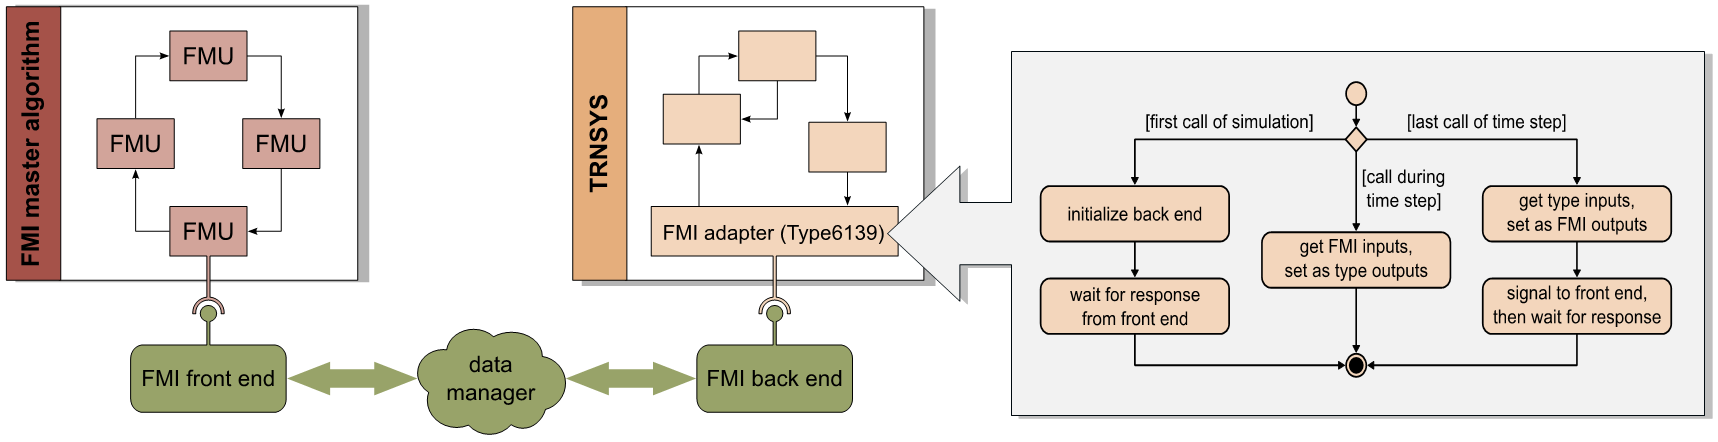
\includegraphics[width=\textwidth]{trnsys_export_schematics}}
\caption{Schematics of \fmipp \trnsys FMU export.}
\label{fig:schematics}
\end{figure}
